\documentclass{ieeeaccess}
\usepackage{cite}
\usepackage{amsmath,amssymb,amsfonts}
\usepackage{algorithm}
\usepackage{algorithmicx}
\usepackage{algpseudocode}
\usepackage{graphicx}
\usepackage{textcomp}

\ifCLASSOPTIONcompsoc
\usepackage[caption=false, font=normalsize, labelfont=sf, textfont=sf]{subfig}
\else
\usepackage[caption=false, font=footnotesize]{subfig}
\fi

\ifCLASSINFOpdf
   \usepackage{graphicx}
   \usepackage{lipsum}
   \usepackage{booktabs}
   \usepackage{threeparttable}
   \usepackage{caption}
   \usepackage{epstopdf}
   \usepackage{cite}
\else
\fi

\usepackage{xcolor}

\def\BibTeX{{\rm B\kern-.05em{\sc i\kern-.025em b}\kern-.08em
    T\kern-.1667em\lower.7ex\hbox{E}\kern-.125emX}}
\begin{document}
\history{Date of publication xxxx 00, 0000, date of current version xxxx 00, 0000.}
\doi{10.1109/ACCESS.2017.DOI-}

\title{Unfolding the City: Spatial Preference Based on Individual Characteristics}


\author{\uppercase{Qi wang}\authorrefmark{1,2}, \uppercase{min lu}\authorrefmark{2,3} and \uppercase{Qingquan Li}\authorrefmark{1,2}}
\address[1]{State Key Laboratory of Information Engineering in Surveying, Mapping and Remote Sensing, Wuhan University, Wuhan 430072, China}
\address[2]{Shenzhen Key Laboratory of Spatial Smart Sensing and Services, Shenzhen University, Shenzhen 518060, China}
\address[3]{School of Architecture and Urban Planning, ShenZhen University, Shenzhen 518060, China}

\tfootnote{This work was jointly supported by the National Natural Science Foundation of China(No. 71961137003 and No. 41671387).}


\markboth
{Author \headeretal: Preparation of Papers for IEEE TRANSACTIONS and JOURNALS}
{Author \headeretal: Preparation of Papers for IEEE TRANSACTIONS and JOURNALS}

\corresp{Corresponding author: Qingquan Li (e-mail: liqq@szu.edu.cn).}

\begin{abstract}
A city is shaped not only by its assembled infrastructures but also the people living inside it. People in a wide range of individual social characteristics visit places with different weights and preferences, sculpturing the city into a space of diverse mobility patterns. Different from the well study of anonymous travel behaviors, the daily movement of characterized individuals, is less studied because of the challenges in collection and analysis of data with privacy. In this work, we take a step forward and perform an online census to collect individual profiles and movements from large-scale volunteers. Then we develop a visual analytic system to investigate the mobility patterns of groups by specifying characteristics. To facilitate the identification of characterized groups, individuals are embedded in t-SNE projection for an abstract overview as well as drawn as vivid graphics by a data-driven profile method for detail examination. A 2.5D spatial visualization is proposed to maintain a compact multivariable analysis by relaxing the z-axis to encode information, such as visiting frequency, demands, traveling distance, etc. Together with the cross-filter and flexible 2.5D interactions, the effectiveness and usability of the system are well demonstrated by a study made in Shenzhen.\end{abstract}

\begin{keywords}
Visual analytics, spatial preference, individual characteristics, data collection
\end{keywords}

\titlepgskip=-15pt

\maketitle

\section{Introduction}
\label{sec:introduction}
\PARstart{T}{he} science fiction \textbf{Folding Beijing}~\cite{hao2016_foldingbeijing} depicts a world where three social classes of people live in independent spatiotemporal patterns, though sharing the same earth surface. This is an artistical metaphor for one potential fact that people prefer to select different places according to individual characteristics, such as social, economic, educational features. This phenomenon has attracted the research interest for a long time in the sociological field. Back to 1970, Pahl~\cite{pahl1975whose} posed the question "whose city" and interest in understanding the territorial inequalities. Contemporary contestation also continually raises the banner "The City Belongs to All!"~\cite{Mayer2017_whosecity}. Having a good understanding of relationships between the spatial attractiveness and the characterized individuals sheds light on region utilization, diversity mix-up, and opportunities promotion.

In the past decades, the power of visual analytics in exploring spatiotemporal data has been recognized and well developed. Various urban problems are answered, such as traffic jams~\cite{wang2013visual}, interchanging flows in public transportation~\cite{zeng2013visualizing}, etc. The presence of social media applications fuels the spatial analysis with rich semantic texts, so researchers get the chances to explore the thematic meaning of the moving behavior, such as events~\cite{chen2017map} or topics~\cite{bosch2013scatterblogs2}. Those works essentially contribute in deepening the contextual understanding of moving activity. However, they rarely combine the movement analysis with individuals' characteristics because which cannot be fully inferred from social media profiles. One of the main challenges is the sensitivity issue in privacy data. There is still a research gap in exploring the relationship between spatial pattern and social characteristics.


In this work, we contextualize the analysis of citizens' spatial distribution in the backcloth of individual characteristics. With the motivation of fusing the movement data with individuals' profiles in an attempt to ascertain the spatial distribution for groups with different characteristics, we need to get the characterized information of movers. The conventional offline census takes lots of effort and too much time to be out of date. With the wide use of the mobile device, it is possible to count information online. In this work, with a census survey released via social media application, we ran an online demographical collection campaign. Based on the data collected, we developed a visual analytics system to explore where do citizens prefer to go. The system incorporates visualizations of individuals' characteristics, including t-SNE for an overview and data-driven profile visualization for the detailed check, as well as 2.5D spatial visualization to explore the distribution of movements. Finally, applying our method in Shenzhen, several cases are derived to demonstrate the powers of our method. There are two contributions of this work:

(1) investigate mobility patterns with characteristics, which is a natural step into research of social understanding of the city.

(2) develop a visual analytic system, whose effectiveness and usability is well demonstrated by a study made in Shenzhen.




\section{Related Work}
This work concerns the research topic of spatial data visual analytics. Spatiotemporal data has three components, i.e., spatial, temporal and thematic~\cite{andrienko2013visual}. Lots of related work focus on the spatio-temporal analysis in movement data, in the absence of thematic information. The presence of geotagged social media data flourishes the exploration of thematic information along with movement. By analyzing the texts, those work explain what drive the moving activities or what is resulted from. This work continues the thematic research in movement data but focuses more on individual characteristics. Landed by a census experiment, this work is able to analyze the profile information directly, to get rid of indirect data inferred from social media data as other related works do.

\subsection{Movement data analysis}
With the development of location-acquisition techniques, massive spatial trajectories are collected, to keep track of the trajectories of various moving objects. Many techniques have been proposed to process, mine trajectory~\cite{Zheng2015_trajectory}. In the field of visualization and visual analytics, spatial visualizations are specifically designed for the time, locations, spatial-temporal information and other properties in the traffic data~\cite{chen2015survey}. A large number of visual analytics tools and applications cover situation-aware exploration, pattern discovery and traffic situation monitoring. Wang et al~\cite{wang2013visual} extract the traffic jam propagation graph extraction to reveal underlying data patterns. Guo et al.~\cite{guo2011tripvista} and Zeng et al.~\cite{zeng2013visualizing} construct geographical regions and visually aggregate the in-between movements as flows. To discover the route travel patterns, Lu et al.~\cite{lu2015trajrank} propose TrajRank to explore the route travel behavior based on ranking. For multiple routes, Liu et al.~\cite{liu2011_routediversity} study the route diversity between locations and Lu et al.~\cite{Lu2017_multipleroute} explore the route choice behavior among multiple routes.

\subsection{Geo-tagged Social Media Data Analysis}
As the presence of social media services, social media data with geo-tags are collected to track people's movements in daily lives. As an analog of remote sensing data in social science research, the geospatial big data has been proposed as social sensing ~\cite{liu2015social}. Hence, analyzing movement information along with rich text has become a hot research area in recent years. Those works infer thematic information from the semantic texts. Cao et al.~\cite{cao2012whisper} propose \textit{Whisper} for tracing the pathways of tweets on a spatial hierarchical layout, to investigate how information flow among multiple places. Krueger et al.~\cite{krueger2014visual} used GPS and location-based service data to support the analysis of movement behaviors. Chen et al.~\cite{chen2016interactive} present a visual analytics system to support the exploration of sparsely sampled trajectory from social media. Some other researchers tend to infer real information, such as names, gender, etc, from social media data~\cite{peddinti2014internet}, to break down the demographic characteristics of social media users. Luo et al.~\cite{luo2016explore} derive race, gender, and age as three demographics dimensions to analyze its impact on the urban human mobility patterns. Since real information is not enforced in social media, the wrong inferring is inevitable. Longley et al.~\cite{Longley2015}~\cite{Paul2016_twitter} identifies and assess the biases inherent in social media usage in social research and evaluate the deployment of social media data in research applications.

\section{motivation}

\label{sec:concept}
This work was sparked from a meeting with two domain experts who work on human mobility and urban informatics in the geospatial field. The experts pointed out that as big and open data evolved in, the scope of urban research has been lifted from the spatial perspective up to social-spatial perspective. There is a rising research interest in understanding how groups of citizens with certain social characteristics select places during their daily lives. Whether people visit places with preference which are intrinsically affected by their social-economic characteristics? Is there a limitation or probabilities of interaction between different socio-economic groups in public spaces? With the advances of data acquisition and analysis techniques, they demanded to go beyond the conventional static sampled questionnaires, which usually survey visiting preferences. They sought for the possibility in revealing the spatial distribution in real-world visiting logs and urged to have a dynamic system which supports the interactive examination of spatial distribution in different contexts of social characteristics.

Thereafter we booted up this project with several rounds of discussions, to frame the research problem with two core contents and the research procedure. The first concepts is \textbf{Social Characteristics}.  Social characteristics of a person or group of citizens  are the descriptors which contribute to the specification of the populations. This work intends to cover the social characteristics from multi-facets, including descriptors such as gender, income, education, etc. The second content is \textbf{Spatial Distribution}. It is reflected by the popularity of a place to be visited.

Motivated by their research interest in understanding the spatial attractiveness with individual social characteristics, this work goes through a procedure consists of two stages, i.e., data collection and basic reviewing, visual analytics design iteration with experts' feedback.

\section{Data Description}
\label{subsec:pipeline}
Considering there is no existing public dataset could fit our topic well, this work is consolidated with a self-maintained data sourcing. We release an online data census to collect the social characteristics and movement logs of individuals for almost half a year. Then a series of statistical analysis is performed on the collected data for sampling bias checking.

\subsection{Online Census}

The advent of mobile sensing techniques and social media applications makes it possible to collect spatial data by apps within the phones. Complementary to the conventional census, it brings the benefit of convenient collections without much manpower and precise spatial locations by GPS instead of semantic description. Meanwhile, it is possible to collective the movement in human inactive time, such as the mid-night.

In this work, we perform the census survey in Shenzhen, which is one of the most modern metropolis in China. The experiment is deployed on Wechat, the most widely used social media mobile application. Fig. \ref{fig:app} shows the data collecting interfaces. For privacy issue, all detailed personal information are desensitized to categorical levels. Considering the main aim on the relationship between spatial distribution of movements and individuals' characteristics, there are two crucial contents to be collected:

\textbf{Individual Characteristics} Fig. \ref{fig:data_over} lists the eight domains, including social, economic and demographic aspects, to give a generalized description of the individual characteristics. The profile will serve as the ingredients for the analysis of mobility patterns over diverse individuals.

\textbf{Traveling Trips} Besides to those individual characteristics, each individual can upload dynamic traveling trips (Fig. \ref{fig:app}(b)). Each trip requires the information of start/end location, start/end time, traveling purpose. To encourage the trip uploading, a credit system retains the contribution of individuals on trips and rewards the volunteers with the top credits (Fig. \ref{fig:app}(c)).


\begin{figure}
 \centering
 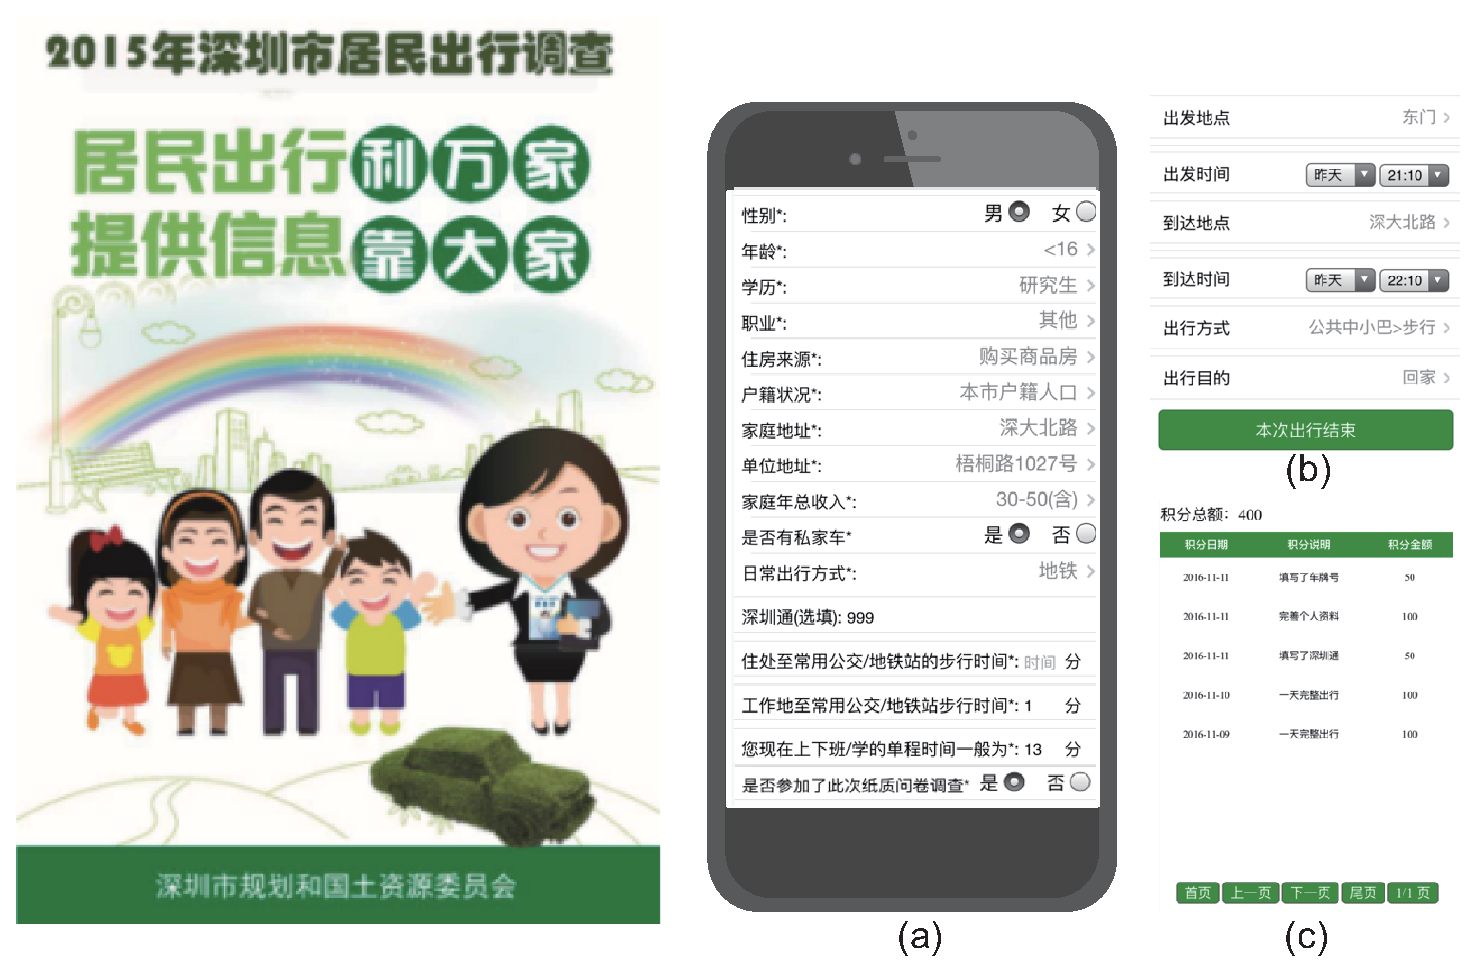
\includegraphics[width=9cm]{pictures/survey_app}
  \captionsetup{justification=centering}
 \caption{Census Interface: (a) personal characteristics collecting page; (b) trips collecting page; (c) credit system page.}
 \label{fig:app}
\end{figure}


\begin{figure}
 \centering
 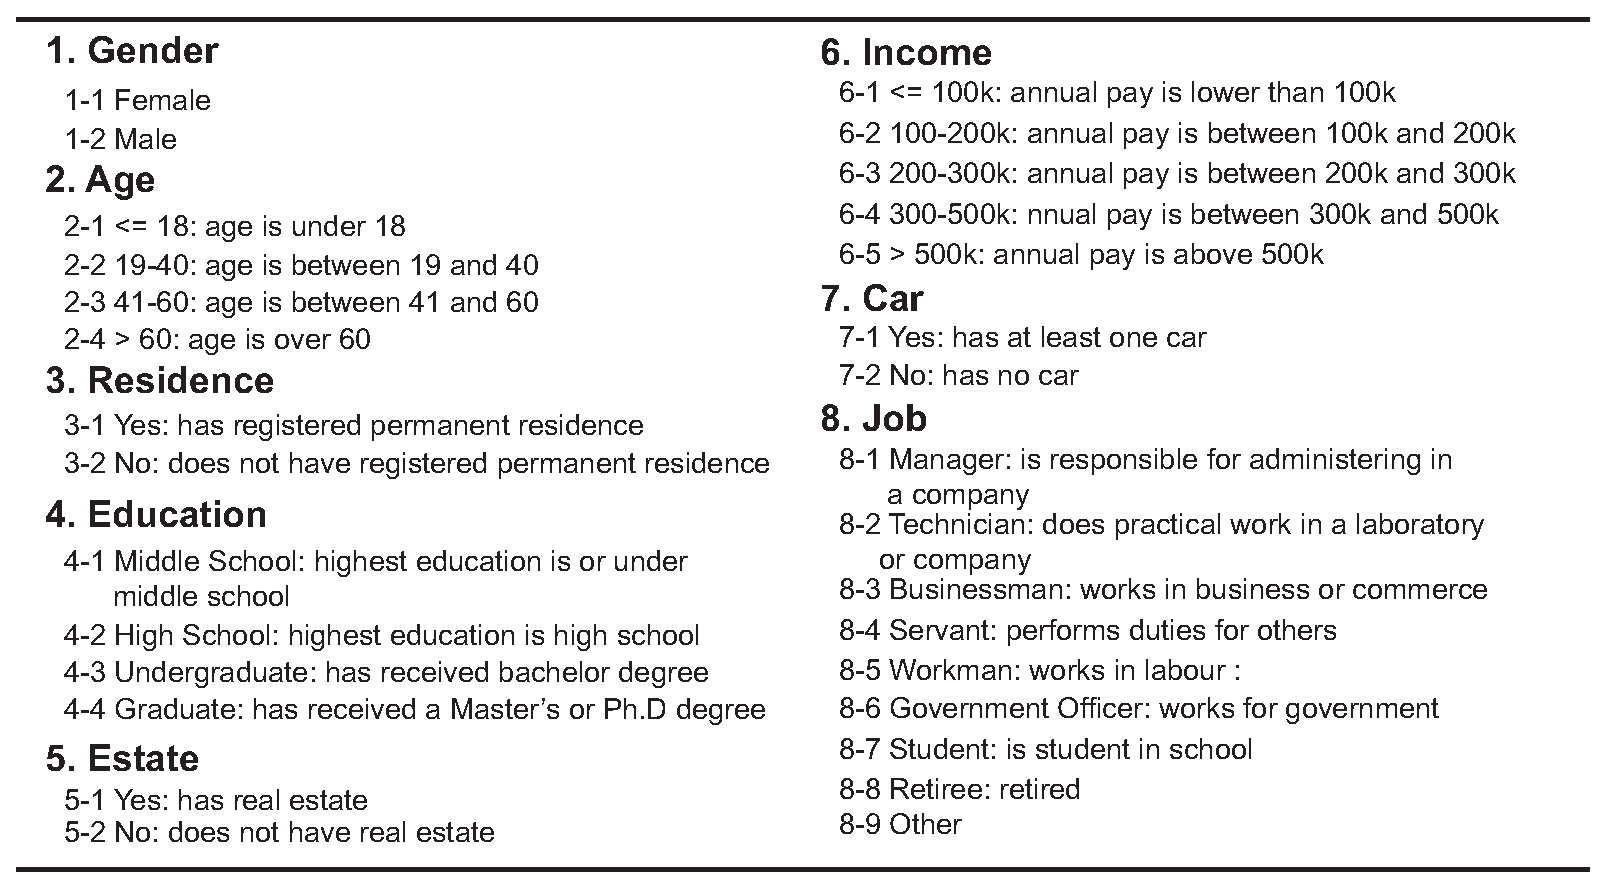
\includegraphics[width=9cm]{pictures/data_over}
 \captionsetup{justification=centering}
 \caption{Profile of Individual: eight individual characteristics enrich the analysis of mobility patterns.}
 \label{fig:data_over}
\end{figure}



\subsection{Statistics of Collected Data}

Over the releasing time period from 2015-11 to 2016-01, 21,435 individuals (48\% females and 52\% males) participated in the census and 229,155 trips were collected. Each volunteer contributed 11 trips average.

\begin{figure}[htb!]
 \centering % avoid the use of \begin{center}...\end{center} and use \centering instead (more compact)
 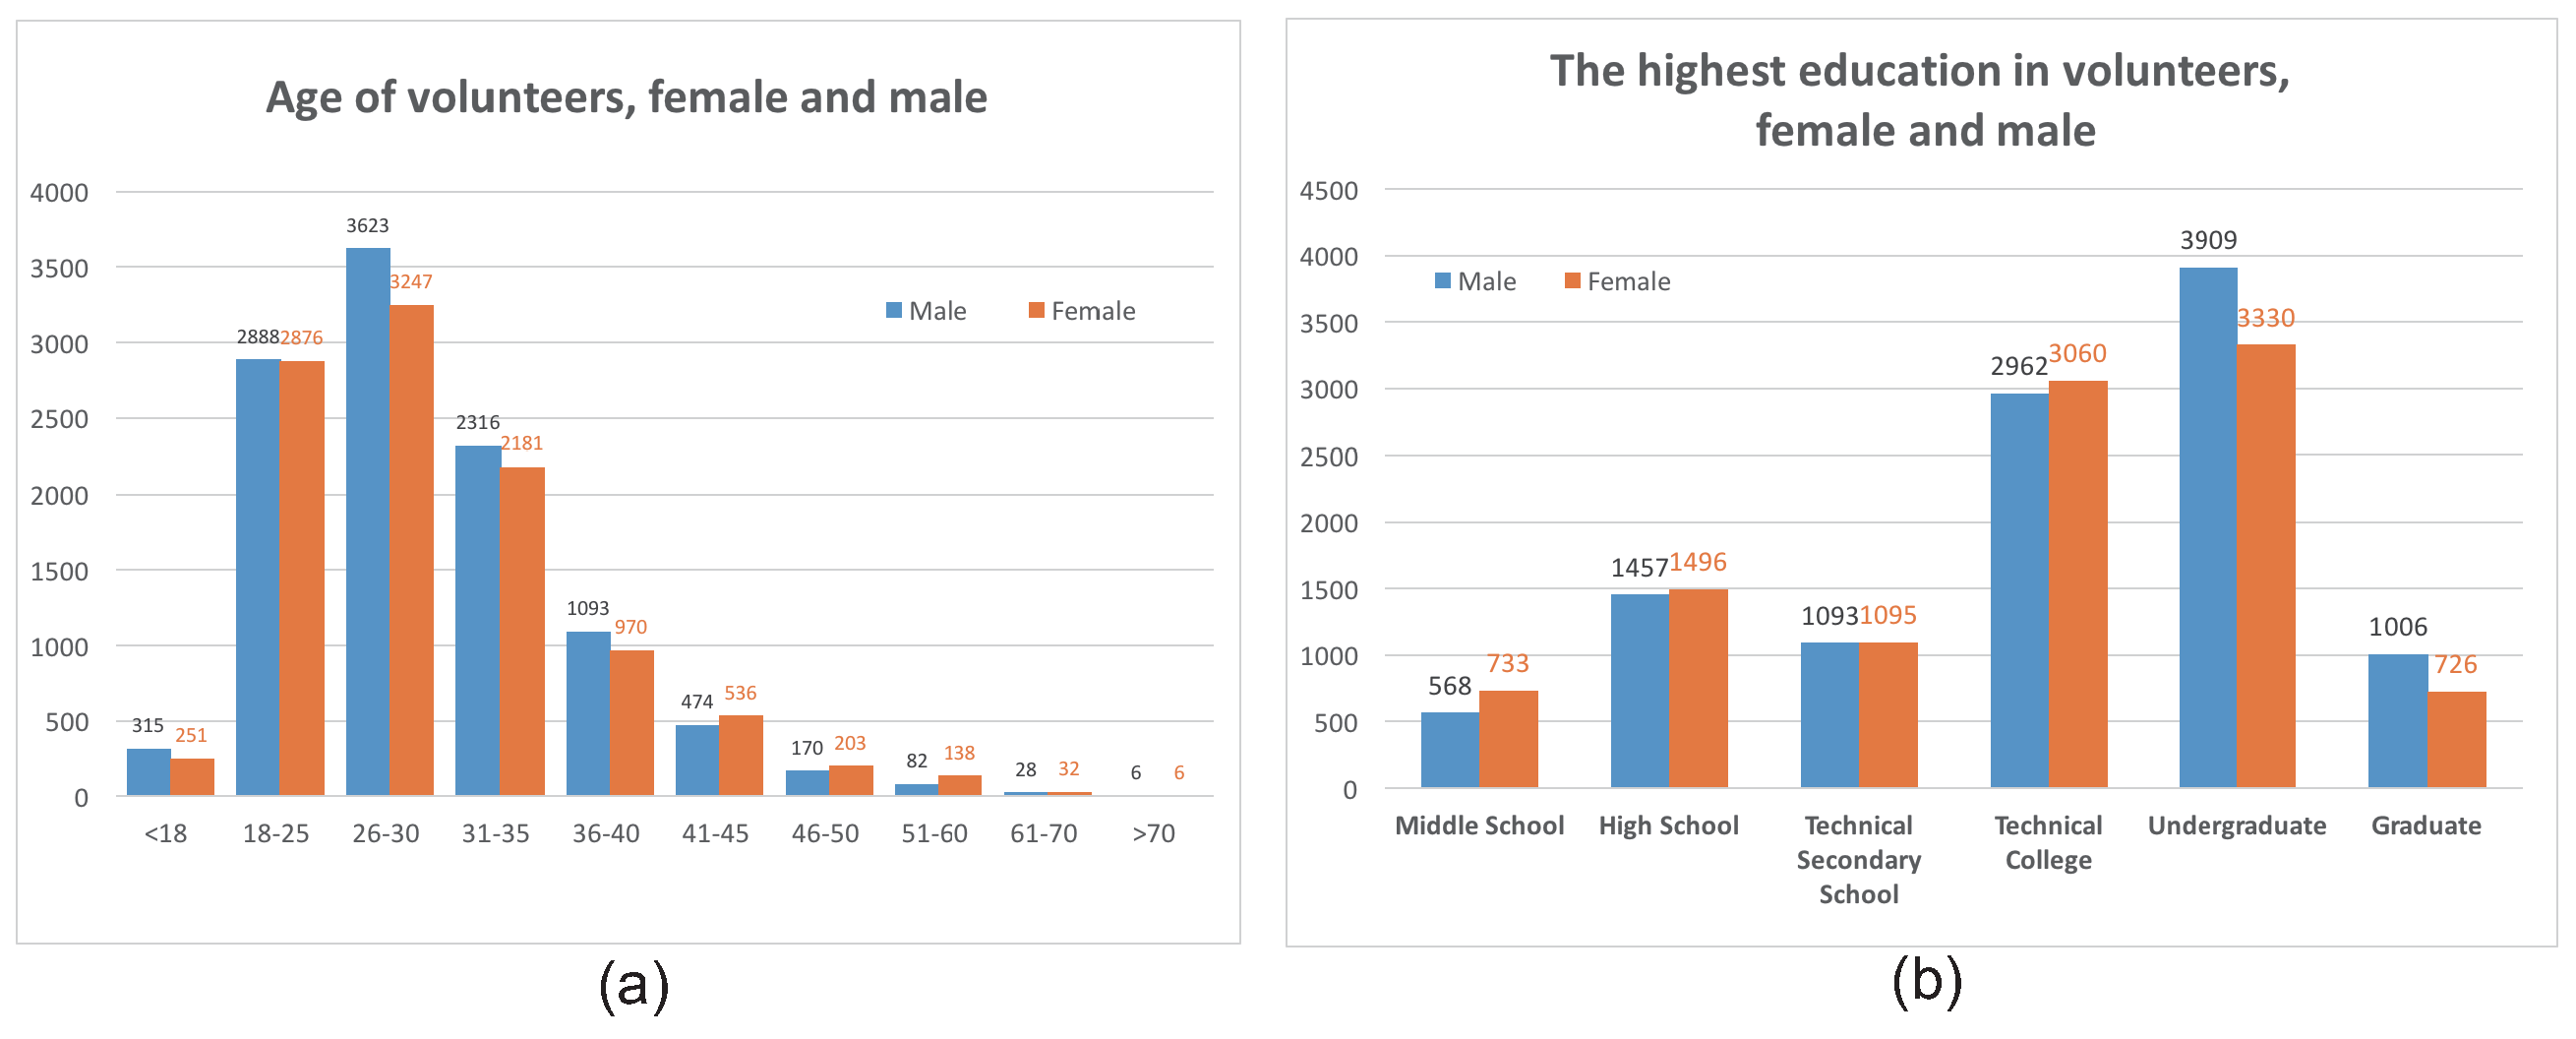
\includegraphics[width=\columnwidth]{pictures/data1}
 \caption{Age and Education Distribution: (a) age; (b) education.}
 \label{fig:data_age_edu}
\end{figure}


Our case-study data is confined to a small proportion of Wechat users who opt to contribute their profile  and movements.
Considering the caveat that self-selecting individuals are most unlikely to represent any clearly defined population~\cite{Longley2015}, we performed a series of preliminary statistics to check whether it is rich enough to represent a wide range of the population in the city.


Fig. \ref{fig:data_age_edu} gives the distribution of age and education over the population. It shows that samples cover a wide range of ages, dominating between 18 to 45. There is also a few records pertaining to individuals below the age of 18 or above 70. The distribution follows the fact that Shenzhen is a city where the majority is young people. According to the 2015 Annual Census Statistics report\footnote{http://www.sztj.gov.cn/xxgk/tjsj/pcgb/201606/t20160614\_3697000.htm}, people aging 15-64 occupy 83.23\% and the median age is 31.5. Fig, \ref{fig:data_age_edu}(b) gives the distribution of education levels, ranging from low to high. The technical college and university dominate the samples at the 61\% occupancy rate.


Fig. \ref{fig:data_job_inc}(a) shows the job types of sampled individuals, who are servants, workers, officers, businessmen and so on. Fig. \ref{fig:data_job_inc}(b) gives the radar diagram of the annual pay. The majority get paid below 200,000. Individuals with higher salary are also reached in our census.

\begin{figure}[htb!]
 \centering % avoid the use of \begin{center}...\end{center} and use \centering instead (more compact)
 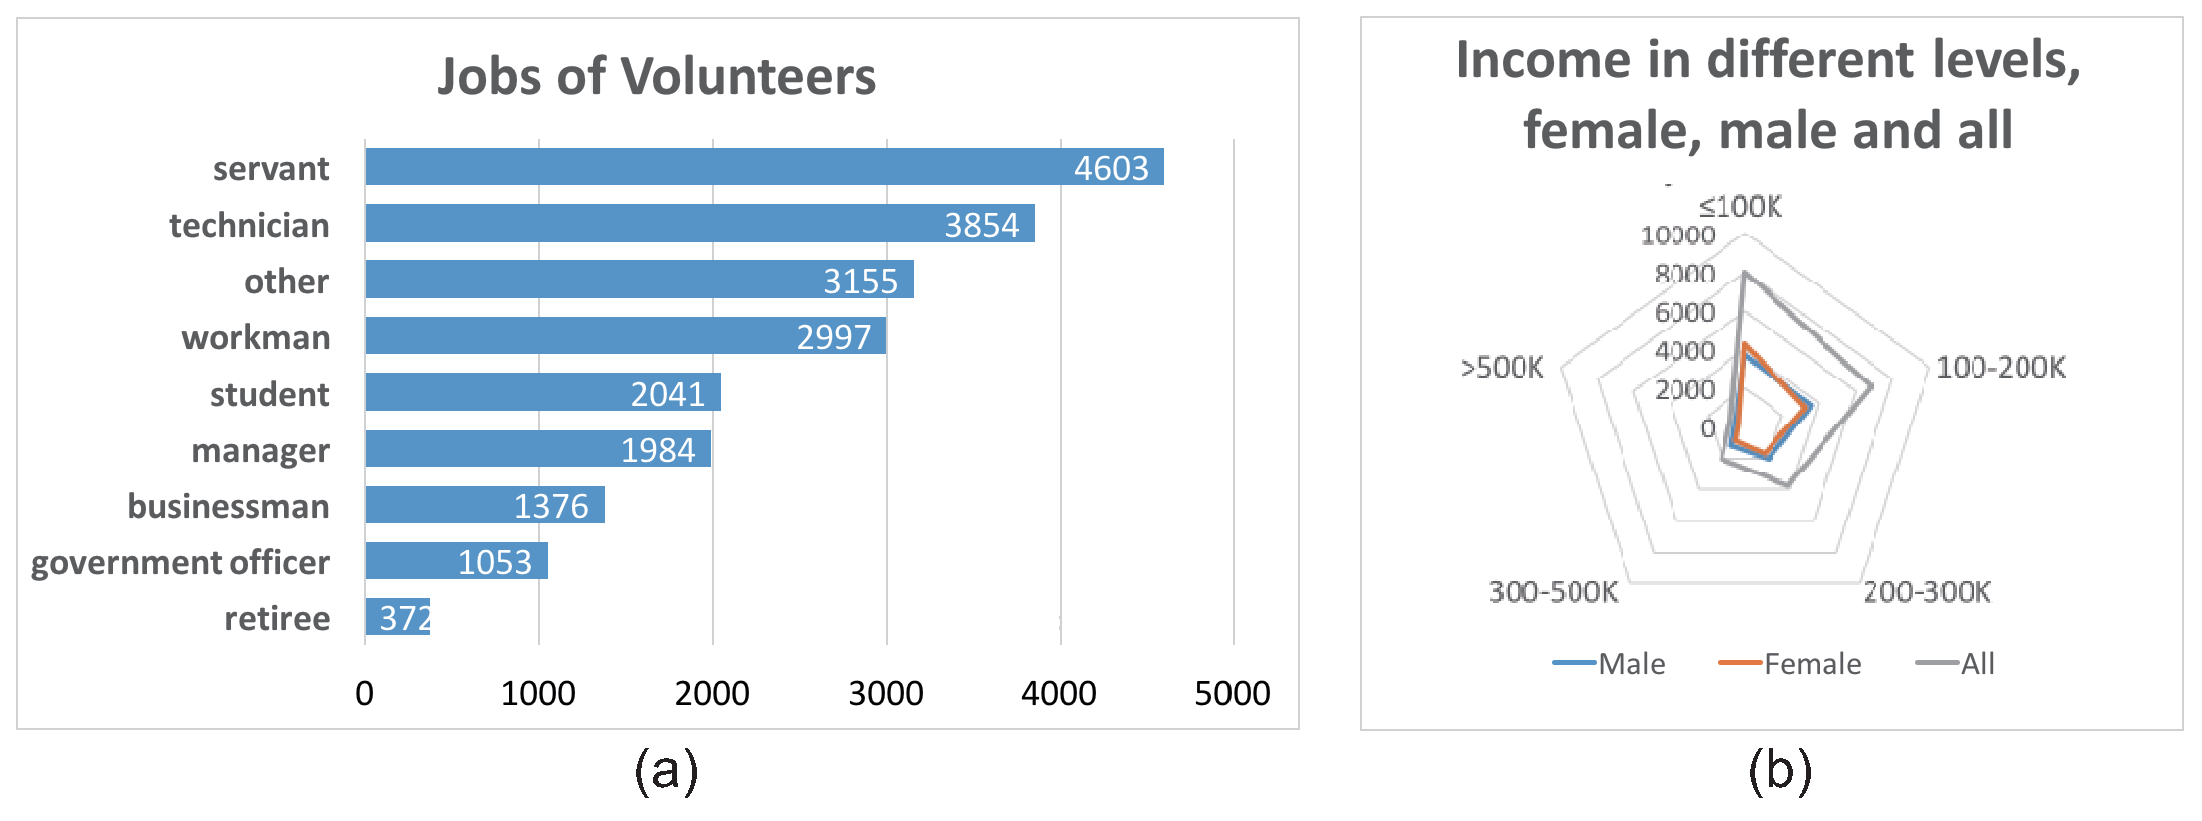
\includegraphics[width=\columnwidth]{pictures/data2}
 \caption{Job and Income Distribution: (a) job; (b) income}
 \label{fig:data_job_inc}
\end{figure}


Fig. \ref{fig:data_geometry} shows the basic statistics related to movements. In Fig. ~\ref{fig:data_geometry}(a), the active traveling time (here, we take the start time as the representative of active time) follows the common knowledge of urban life. There are obvious morning and late afternoon peaks. Fig. ~\ref{fig:data_geometry}(b) gives the counting of different traveling purposes. 95\% trips are tagged with clear raveling purpose in the data. 33\% are going home and 37\% are going to work. Besides this kind of routine traveling, there are also substantial trips such as going shopping, going the hospital, etc. Fig. ~\ref{fig:data_geometry}(c) shows the spatial distribution of the origins and destinations. It is found that more dots are located in Futian and Nanshan districts, the city's heart than the surrounding areas. This is consistent to Batty's exposition of the focus of city networks and interaction patterns~\cite{batty2013new}.

\begin{figure}[htb!]
 \centering % avoid the use of \begin{center}...\end{center} and use \centering instead (more compact)
 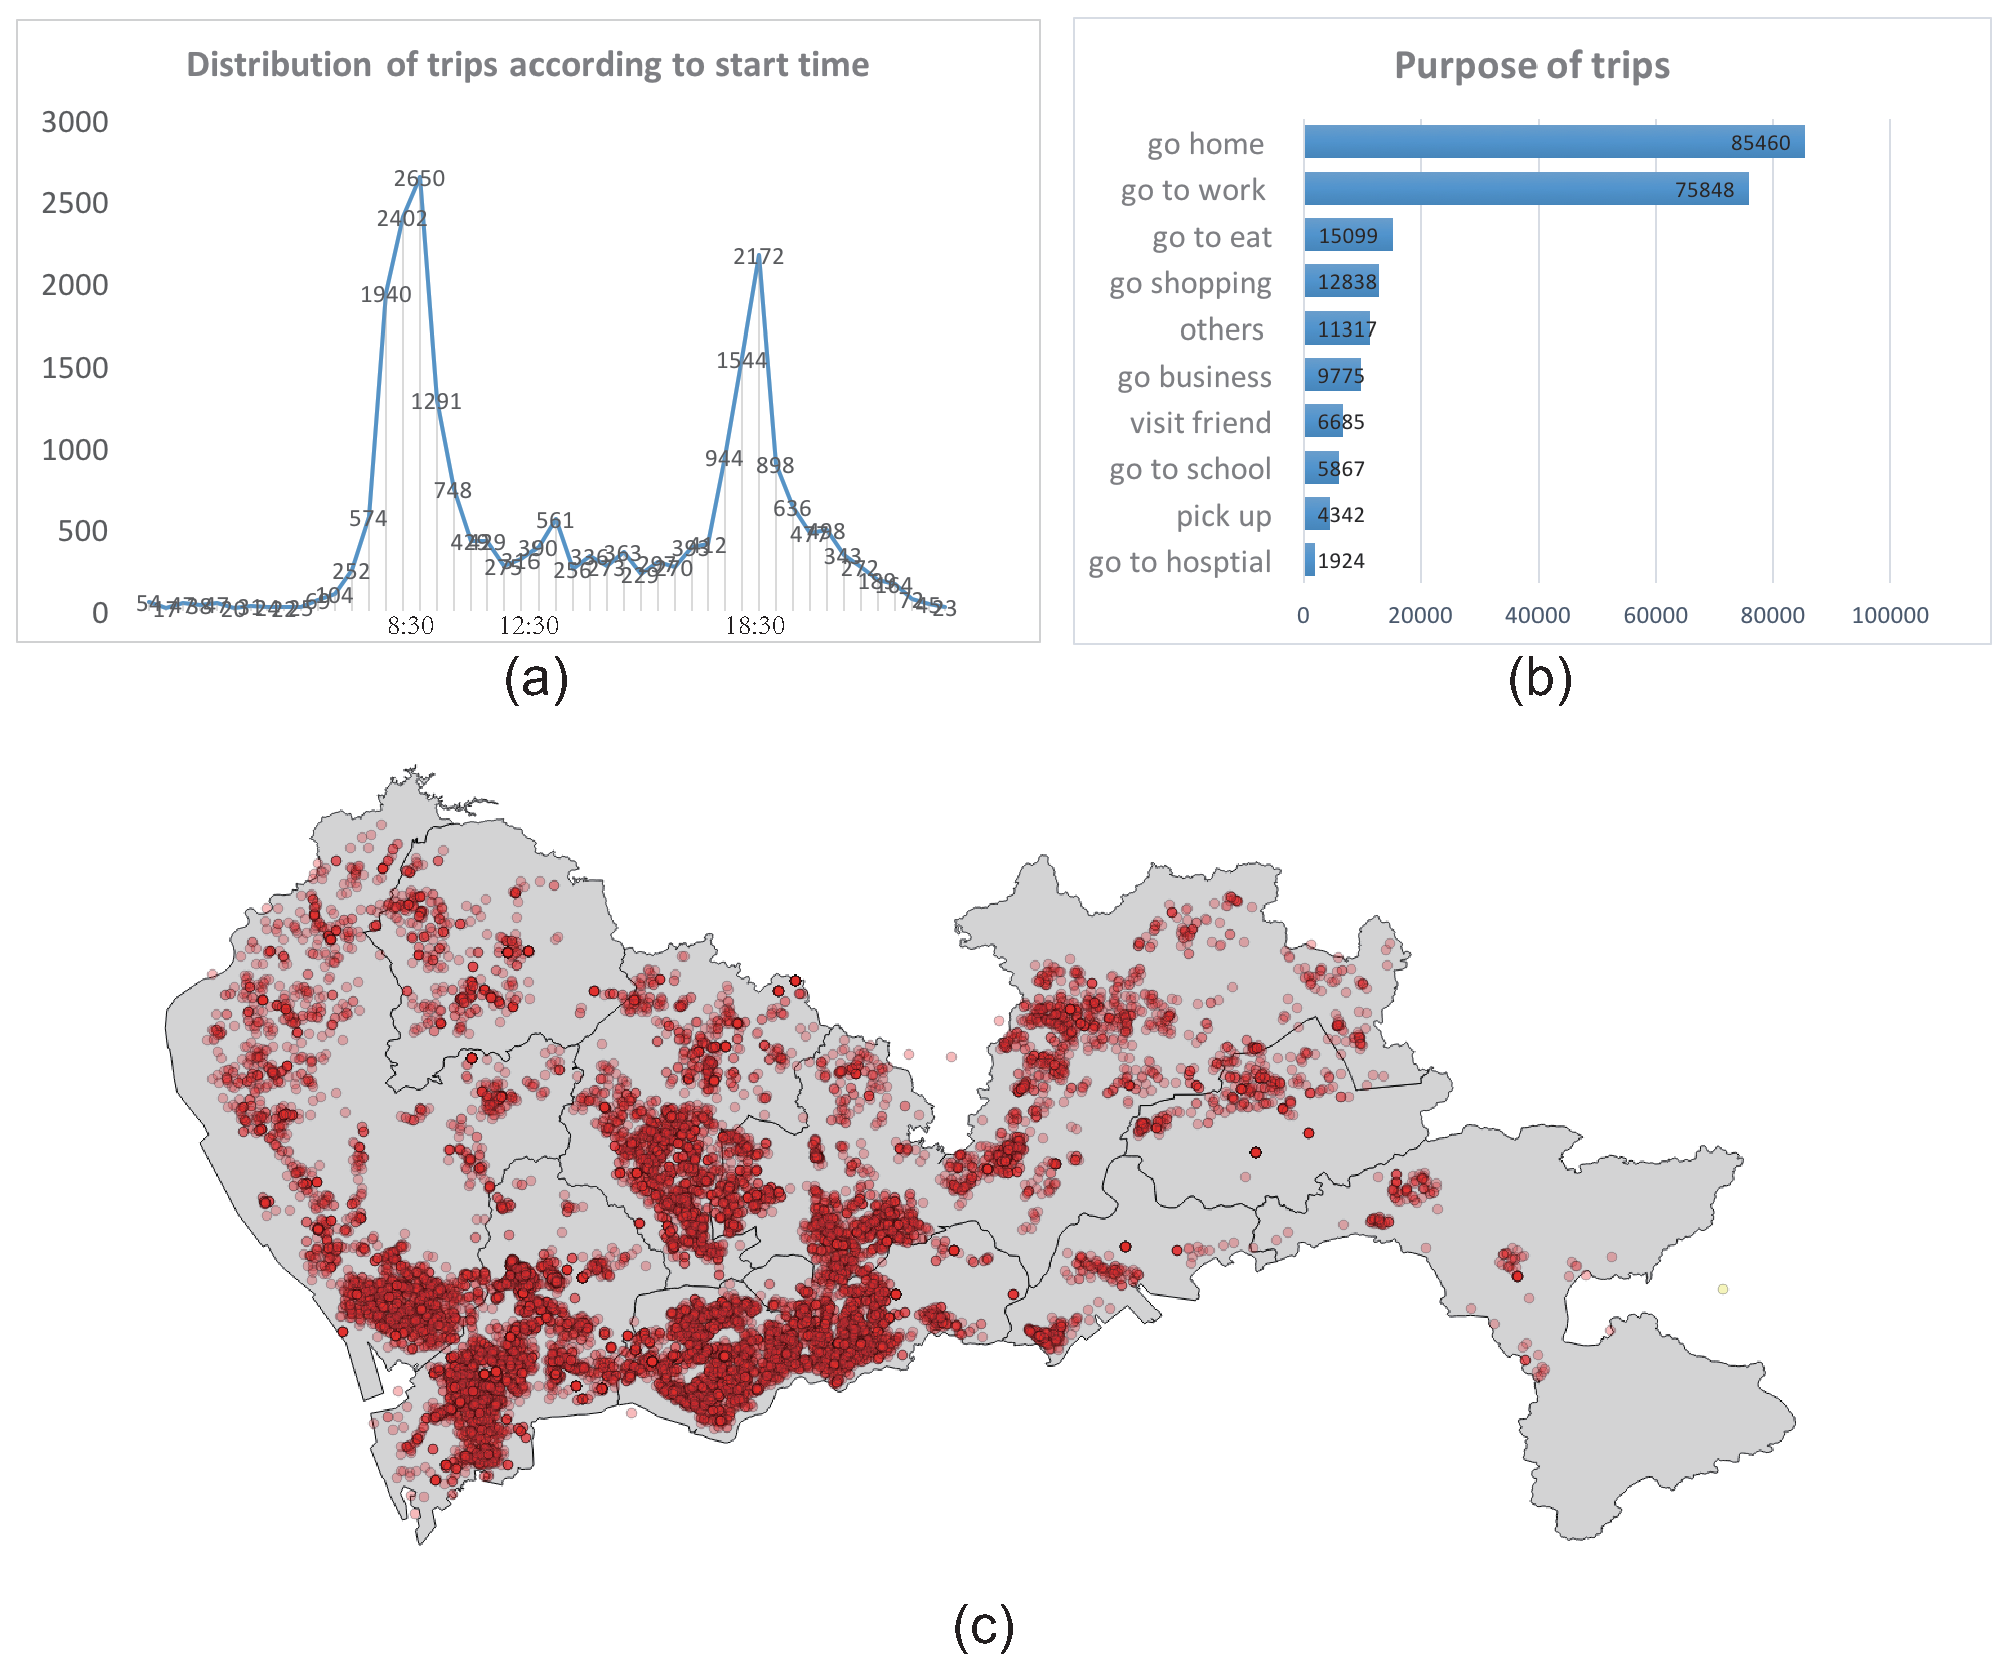
\includegraphics[width=\columnwidth]{pictures/data3}
 \caption{Statistics of Trips: (a) start time of trips; (b) purpose of trips; (c) distribution of origins/destinations }
 \label{fig:data_geometry}
\end{figure}

Because there is always inevitable bias inherent in fully representing the ground truth of the population, the preliminary statistical analysis shows positive sign of a relatively even sampling of the population.

\section{Visual Design}

The design of visual analytics system is iterated via multi-pass discussions with the two domain experts. In this section, we first introduce specific tasks the system intended for and design rationales aligned to provide the user-friendly interface for domain experts. Then we introduce the visual design.

\subsection{Tasks}

The exploration of core contents (introduced in Section~\ref{sec:concept}) is resolved further with the following tasks.

\begin{itemize}
\item \textbf{Task 1: Identify the group with specific individual characteristics}: to get groups of people with common or close attributes, to explore the correlation among individual characteristics.
\item \textbf{Task 2: Explore the mobility distribution of a group}: to explore where, how and why an interested group go in the city.
\item \textbf{Task 3: Compare mobility distribution among multiple groups}: to know the similarities and differences between different groups in their spatial preferences, to investigate the relationship between movement and individual characteristics.
\end{itemize}

\begin{figure*}[htb!]
 \centering % avoid the use of \begin{center}...\end{center} and use \centering instead (more compact)
 \includegraphics[width=18.1cm]{pictures/teaser.eps}
 \caption{System Interface: (a) an interactive infographics provides the basic statistic facets of individuals; (b) a t-SNE visualization gives an overview of individuals, where the similarity in high dimensional space is preserved in 2D space; (c) data-driven profiles support users with organic individual perception; (d) group of interested individuals can be saved; (e) movement of the chosen group is visualized and explored in 2.5D main view; (f) a dock is provided to restore and compare findings; (g) different choices of 2.5D encoding can be selected.}
 \label{fig:teaser}
\end{figure*}

\subsection{Design Considerations}

With these three tasks, we derive following design considerations:

\begin{itemize}
\item \textbf{Intuitive perception of an individual as an organic complex (C1)}: the system should make use of users' daily life experience in knowing people to provide intuitive visualization, instead of the lifeless representation by number. The visual design needs to help end-users to pick desirable ones from the mass.
\item \textbf{Good overview of the multivariate individuals (C2)}: following the visual analytics manta by Shneiderman~\cite{RN459}, it is very important to provide a good overview of all the individuals then the users know where to explore.
\item \textbf{Effective multivariable cross-filter for individual characteristics (C3)}: there are eight domains to describe an individual. The system is supposed to provide a straight-forward way for easy filtering by the eight criteria.
\item \textbf{Compact visualization of mobility patterns in the constraint of spatial space (C4)}: the analysis of mobility patterns not only includes the conventional spatial and temporal dimensions, but also other abstract dimensions, e.g., travel purpose, visiting frequency, etc. The system should handle a compact layout to support the easy correlation between spatial and abstract information.
\item \textbf{Flexible interactions to explore the mobility patterns either within one group or between groups (C5)}: to support the comparison among groups, \textbf{Task 3}, the system should maintain flexible interactions which allow the end-users to explore freely.
\end{itemize}




\subsection{Visualizations}
\label{subsec:vis}

With those design considerations, we develop a visual analytics system as Fig. \ref{fig:teaser} shows. It composes of individual panel (the left part) for individuals (\textit{Task 1}) and spatial panel (the right part) for the mobility pattern (\textit{Task 2 and 3}). In the individual panel, interactive infographics, t-SNE visualization, and data-driven profiles support users to narrow the scope down to groups of individuals with interested characteristics. With the chosen group of individuals, its moving related information is visualized and explored in a 2.5D spatio-temporal view.



\subsubsection{Data-driven Profile Visualization}

Glyph-based visualization~\cite{borgo2013glyph} is the form of visual design to compose multivariable into a collection of unified visual symbols, known as a glyph. A glyph is intended for quick understanding and aligned comparison. Among glyph design, Chernoff Face~\cite{chernoff1973use} represents data variables by the different features of a cartoon face. Following the idea of Chernoff Face, we design a type of glyph, a graphical representation of people with specific individual characteristics. The idea behind using faces is that humans easily recognize faces and notice small changes without difficulty (\textit{C1}). Those visual profiles are intended for intuitive visual understanding, from abstract to concrete and semantic understanding, to support users to target the interested individual groups effectively.

Fig. ~\ref{fig:design_profile} shows the legend for the user profile. The eight domains are encoded by visual symbols and organically organized in a human figure. There are basically three types of variables to drive the figure, i.e., the numeric, categorical and boolean ones. For numeric attributes such as income and education levels, visual symbol keeps consistent design but with changing visual variation, such as size, thickness. For the categorical attributes such as job, visual symbols are designed separately for better semantic meaning. For the boolean attribute like car, house, a symbol is designed to indicate its existence. With this consideration, the domains are designed as follows:


\begin{itemize}
\item \textbf{Gender} It is visually mapped to the hairstyle of the avatar.
\item \textbf{Age} Age is implied by the decoration on the hair. For the elder above 70, the hair is dyed to grey. For the youth beneath 18, a hair decoration is adapted for the different hairstyles of girls and boys.
\item \textbf{Education} The thickness of eyeglasses is used to indicate the different levels of education.
\item \textbf{Job} The clothes is designed to imply the job of the individual. There are 9 types of clothes.
\item \textbf{Belongings} For real estate, car, residential license are considered as the belongings to the individual, so we design each of them as an add-on decoration to imply whether the individual has it or not.
\item \textbf{Income} A money symbol is used to represent the income, whose size encodes the income level. The more money an individual earns, the larger the symbol is.
\end{itemize}

\begin{figure}[htb!]
 \centering % avoid the use of \begin{center}...\end{center} and use \centering instead (more compact)
 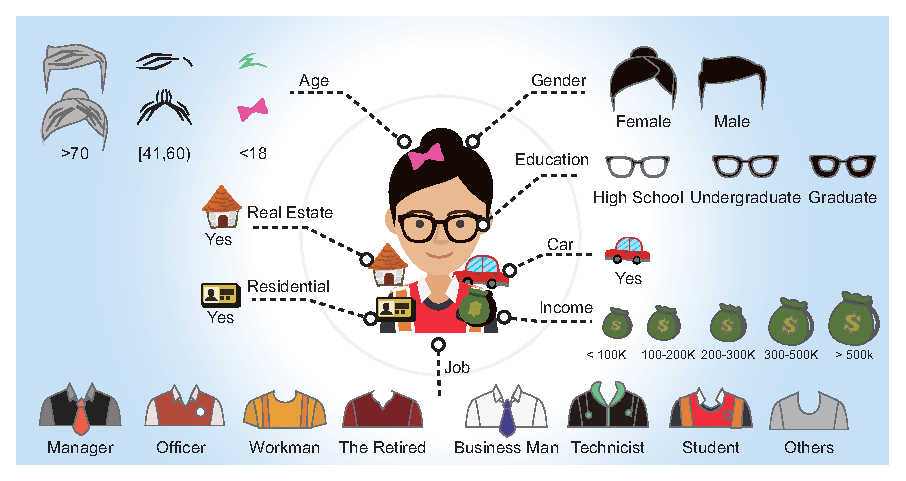
\includegraphics[width=\columnwidth]{pictures/design_profile}
 \caption{Design Profile: the eight characteritical domains are encoded and organized in an organic human figure.}
 \label{fig:design_profile}
\end{figure}

With the visual mapping, the profile varies from individual to individual. By concretizing the attributes which otherwise is too abstract to percept, users can scan and search for interesting target effectively. Fig. \ref{fig:div_example} lists the figures with the top 10 largest population in some job. The textual number beneath indicates the population. It is found that the majority of workmen earn a low salary and most of them have no residential license. On the contrary, for the officers, all of them have the residential license and most of them have a house. Some of the retired people are in old age. Most of the managers are at undergraduates, even graduates.


\begin{figure}[htb!]
 \centering % avoid the use of \begin{center}...\end{center} and use \centering instead (more compact)
 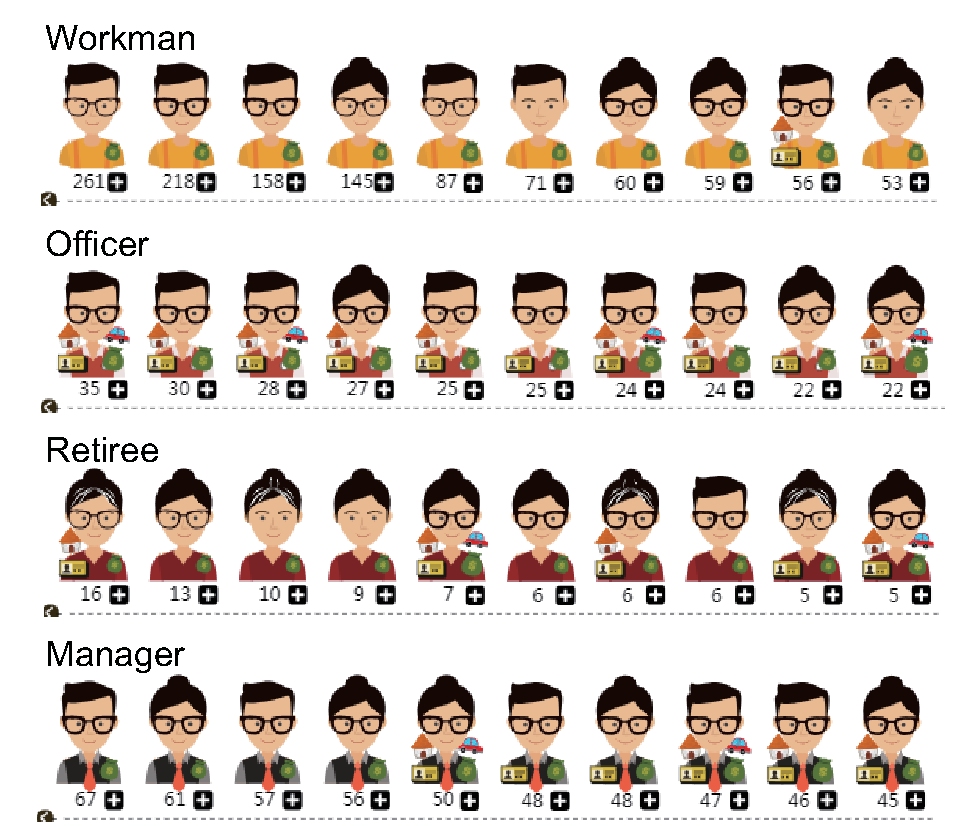
\includegraphics[width=\columnwidth]{pictures/design_example}
 \caption{Representative figures with the top 10 largest population in four jobs}
 \label{fig:div_example}
\end{figure}

\subsubsection{t-SNE Projection of Individuals}

In our case, each individual can be denoted as a vector $x_i$ with eight factors, and we get high dimensional data set $X={x_1, x_2, ..., x_n}$. The dimensionality reduction techniques are to preserve the local structure of high dimensional data in low dimensional space, which are efficient approaches to provide a good overview of the multivarible individuals (\textit{C2}). We adapt t-SNE project~\cite{maaten2008visualizing} to project $X$ as two-dimensional dots $Y={y_1, y_2, ..., y_n}$. One of steps in t-SNE is to compute the conditional probabilities to represent the similarity based on the distance between high dimenional datapoints. The conditional probability $p_{j\mid i}$ between $x_j$ and $x_i$ is given by:

\begin{equation}
p_{j\mid i} = \frac{exp({\left \| x_i - x_j \right \|}^2/2\alpha_i ^{2})}{\sum _{k\neq i}exp({\left \| x_i - x_k \right \|}^2/2\alpha_i ^{2})}
\end{equation}

where $\alpha_i$ is the variance of the Gaussian that is centered on $x_i$. Specifically in our context, the high-dimensional Euclidean distances $\left \| x_i - x_j \right \|$ between $x_i$ and $x_j$ needs to be adpated the numerical and categorical characteristics. Characteristics such as age, income, are numerical and comparable, so the difference exactly explains when they are different. But the other characteristics, i.e. job, real estate, car, residential, are ordinal. There is not the numeric order. For example, the job distance from a manager to a businessman and a workman is not comparable, which is considered the same distance, i.e., set to 1.

As Fig. ~\ref{fig:tsne} shows, all 21435 volunteers are embedded in the 2D view, where the closer two dots are, the more similar they are in the eight characteristics. Fig. ~\ref{fig:tsne} exemplifies four features groups of dots in a neighbor.

Multiple views of abstract view, t-SNE protection, and semantic data-driven profile visualization are coordinated in a Cross-filter mechanism~\cite{Weaver2010}. It allows end-users to interactive drill-down into individuals with interested characteristics from multiple perspectives(\textit{C3}). Starting from the abstract criterion constraints, the scope of interest is narrowed down to individuals with(out) certain characteristics. And then further cross-filtering with semantically visual profiles can be performed to check the combination of 8 characteristical variables.

\begin{figure}[htb!]
 \centering % avoid the use of \begin{center}...\end{center} and use \centering instead (more compact)
 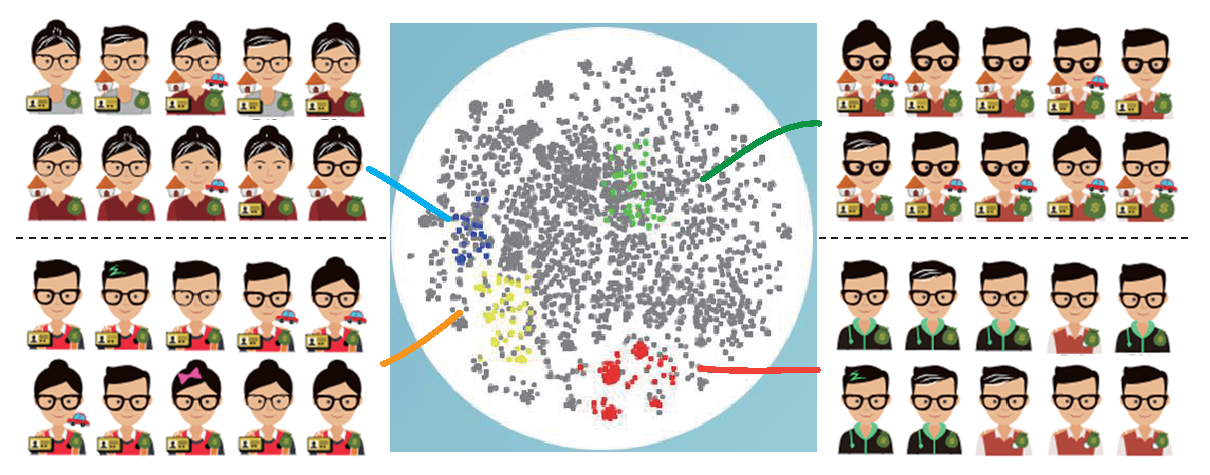
\includegraphics[width=\columnwidth]{pictures/tsne}
 \caption{t-SNE project with four groups of the interest: (a) t-SNE project }
 \label{fig:tsne}
\end{figure}

\subsubsection{2.5D Spatial Visualization}
\label{subsec:25D}


Embedding multiple variables in the spatial map is a challenging problem. Distorting 2D spatial for better space usage, such as the partial route embedding~\cite{sun2016embedding} is an effective method when there are a few local foci. When it comes to the global visualization, there is always a trade-off between occlusion-free and the compact spatial perception. Following the idea of stacking 2.5D space design~\cite{Tominski2012_stacking}, the space in this work is embedded in 2.5D space, to relax the z-axis for additional abstract information encoding.

Fig. ~\ref{fig:2.5D}(a) shows the 2.5D visualization. The spatial map consists of Traffic Analysis Zone (TAZ), which is the unit of geography holding a certain number of people. For the 2.5D, each TAZ is grown as a prism whose height and color are developed to encode abstract information, e.g., the occurrence of visiting. With difference encoding choices, it is capable to visualize the correlation between spatial and different attributes (\textit{C4}). For example, in Fig. \ref{fig:2.5D}(a), prisms' height and color both encode the ratio of none-routine trips (such as go entertainment, go hospital, etc.) in the whole. For better 3D visual perception, lighting is turned on. Also, a lid is laid on the top of each prism to clearly bound its extent at the z-axis.

\begin{figure}
    \centering
	  \subfloat[]{
       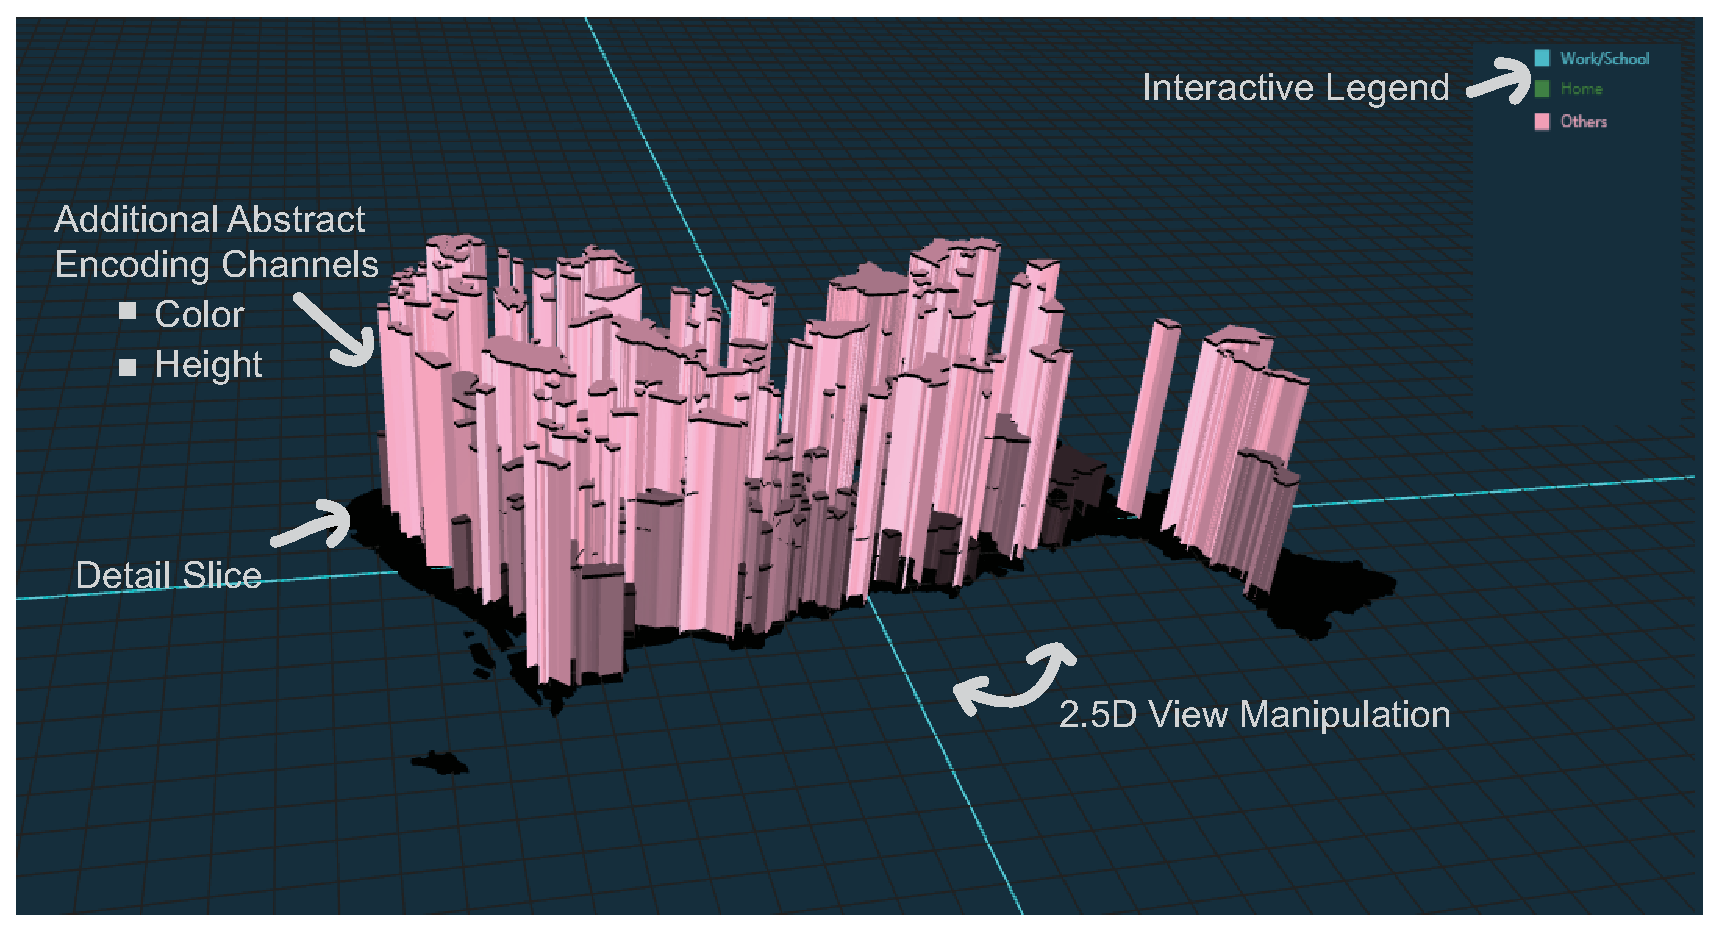
\includegraphics[width=86mm]{pictures/space1.eps}}
    \label{1a}\hfill
	  \subfloat[]{
        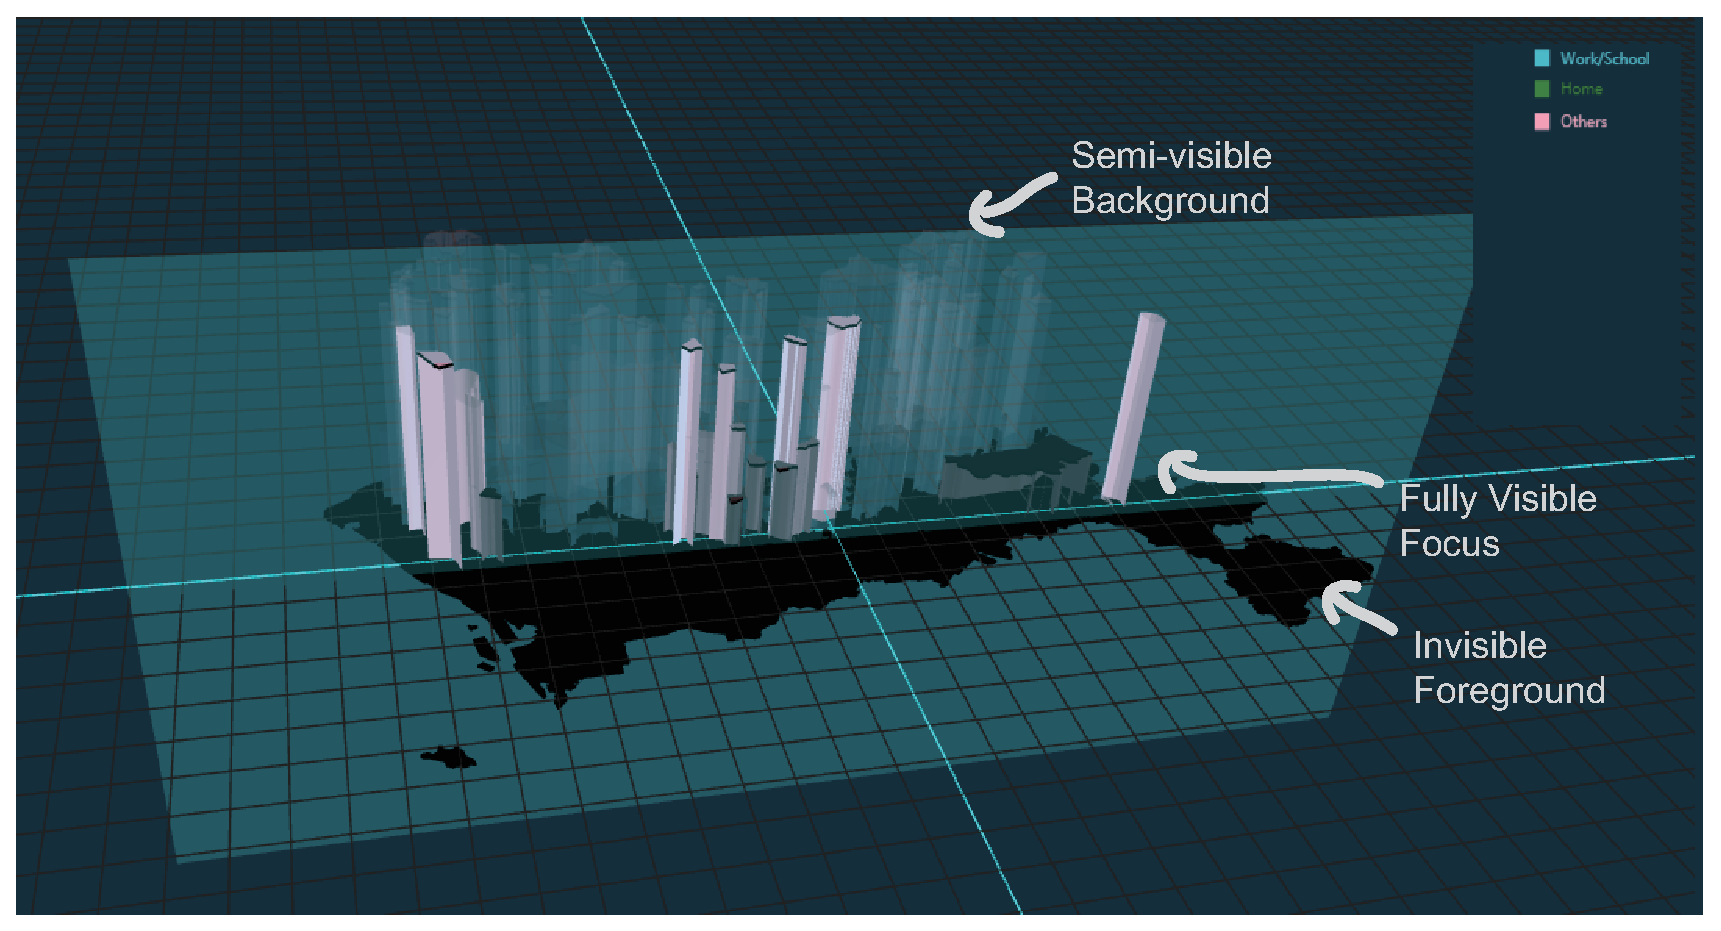
\includegraphics[width=86mm]{pictures/space2.eps}}
    \label{1b}\\
\caption{2.5D Spatial Visualization: (a) 2.5D spatial visualization with z-axis to encode addition information; (b) detail slicing in 2.5D space.}
\label{fig:2.5D}
\end{figure}


Several interactions are integrated into the spatial view to alleviating the occlusion problem (\textit{C5}). The manipulation of 2.5D view supports users with rotate, zoom, pan operations, which are so continuously flexible that users probably find a suitable observing point. In the cases where occlusion is inevitable, an interaction named as \textbf{Detail Slicing} is developed, as Fig. ~\ref{fig:2.5D}(b) shows. Detail Slicing is the operation to put a cross-section in the 2.5D space to expose the TAZ inside. To contextualize the cross-section, TAZs are visually adapted according to the intersection by ray casting. The TAZ in the foreground will be hidden, the intersected TAZs will be fully visualized and the ones in the background will be in semi-transparency.

 To compare the mobility patterns across different groups of people, a Small Multiple dock is used to reserve the ever explored interesting result (Fig. ~\ref{fig:teaser}(f)). To simply the comparison over spatial distribution, the snapshot is also rendered in the 2.5D space, which maintains the same interactions as the main 2.5D space does.


\section{Case studies}

In this section, we apply the method described above to study the case of Shenzhen. We introduce the several cases to demonstrate the usage and effectiveness of the system.

\subsection{Case 1: Home-life distribution VS Income/education}

This work is inspired and motivated by the implication in science fiction~\textit{Folding Beijing}, which is that people are categorized into three classes and behave in the parallel spatial-temporal patterns. The first cast explores whether the folding city exists in reality or not.

\begin{figure}[htb!]
 \centering
 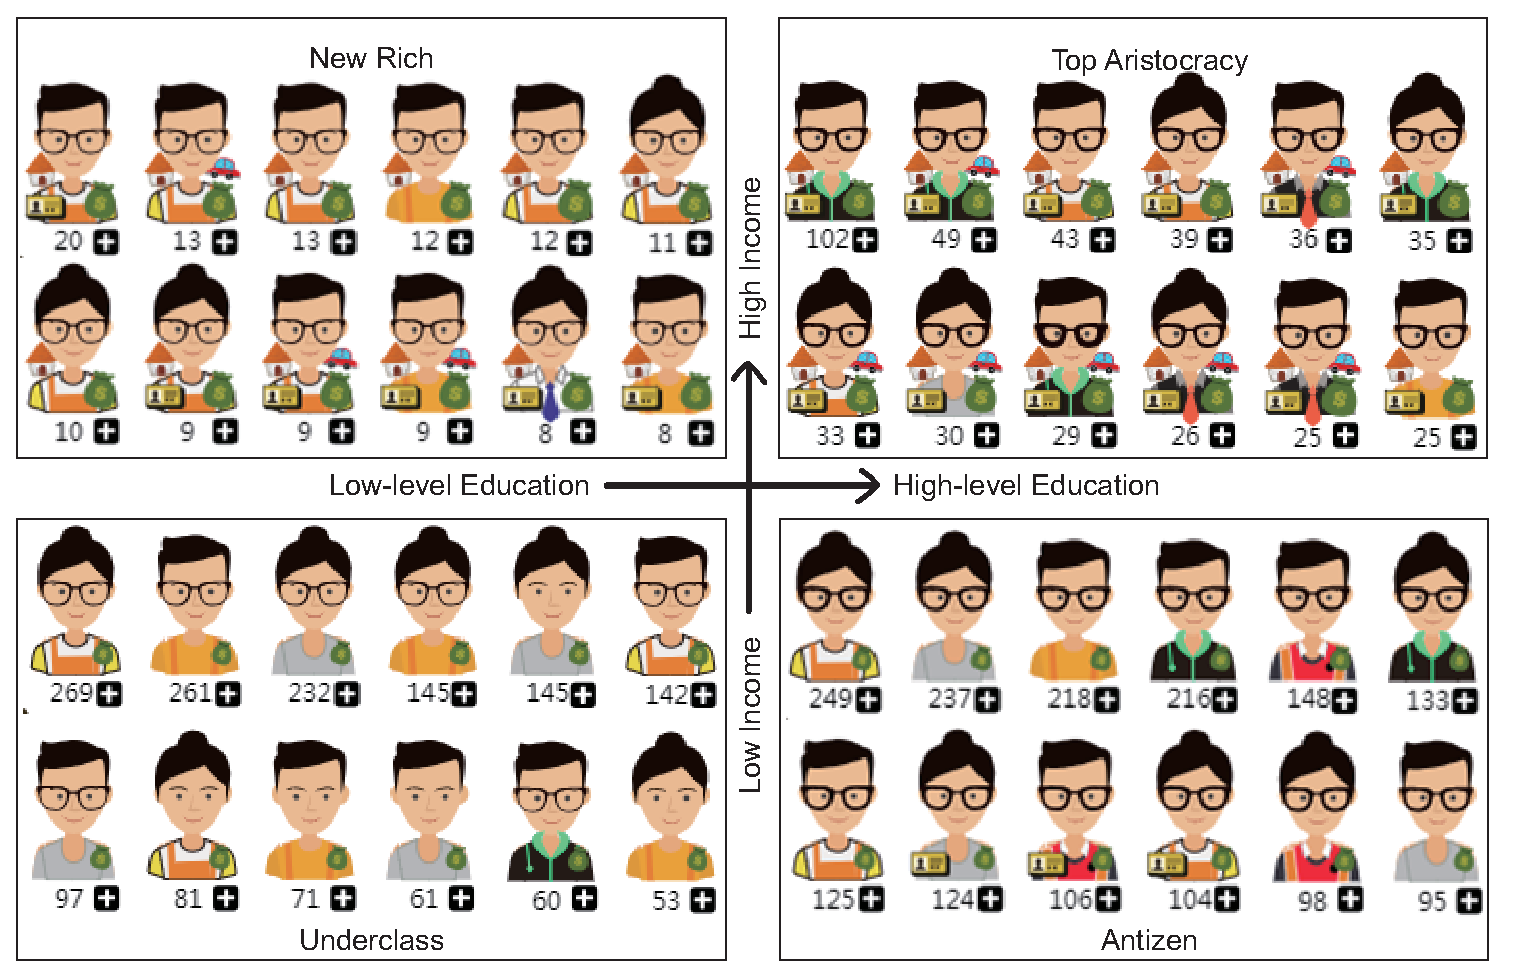
\includegraphics[width=\columnwidth]{pictures/case1_1}
 \caption{Four Groups Divided by Income and Education Characteristics}
 \label{case11}
\end{figure}

Although it is incomplete, income and education are two of the most essential characteristics to tag an individual with a good resource or not.
As Fig. ~\ref{case11} shows, taking income and education as the two dimensions, taking 300,000 yuan as the border between high and low income and an undergraduate bachelor degree as the border between high and low education level, four different groups are generated in the four quadrants. In the first quadrant, individuals are rich and well educated, who are in a group of so-called \textbf{top aristocracy}. The second quadrant holds the group of \textbf{new rich}, i.e., individuals with high income but low education income. In the third quadrant, they are the \textbf{underclass} who has both low income and education level. The fourth quadrant is \textbf{antizen}, which is a new word to describe people have a good education but earn little.


Fig. ~\ref{case11} shows the top 12 profiles with the maximum population in each group. In each group, other characteristics surprisingly demonstrate the high correlation to income and education. For example, almost all of the \textbf{top aristocracy} is with the residential license,  house, and car. On the contrary, \textbf{underclass} do not have the residential license residence, neither the house nor the car. Most of \textbf{new rich} has a house and work in the service industry.

Before diving into the complex mobility pattern analysis, we explore the home distribution of the four groups. As Fig. ~\ref{case12} shows, \textbf{top aristocracy} and most of \textbf{new rich} live concentrated in the downtown area of Shenzhen, where the living cost is higher, especially the housing cost. A small part of \textbf{new rich} lives far away from the downtown, maybe because they don't have to work in downtown. The \textbf{underclass} distribute more dispersively all over the whole city. Compared to the rich, they prefer the outer space because of the lower living cost. Lots of \textbf{antizens} live in Nanshan District, where there are many universities and high-tech industrial parks full of well educated people.

\begin{figure}[htb!]
 \centering % avoid the use of \begin{center}...\end{center} and use \centering instead (more compact)
 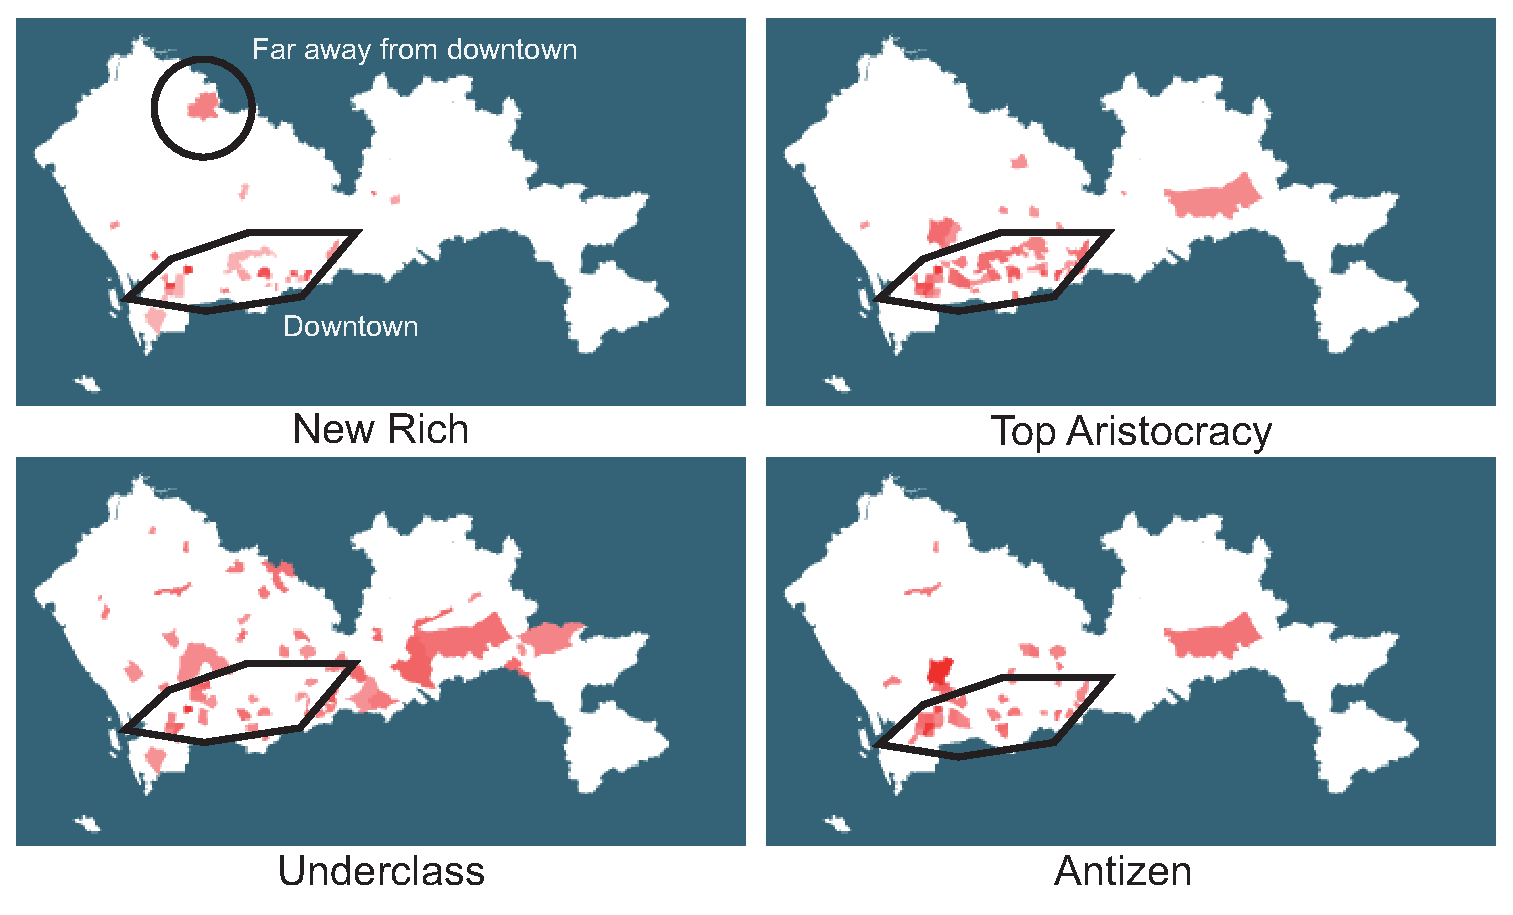
\includegraphics[width=\columnwidth]{pictures/case1_2}
 \caption{Home Distributions of the Four Groups}
 \label{case12}
\end{figure}


To have a better knowledge of mobility patterns of the four groups, trips are categorized into three categories, ``home", ``work'' for regular trips with the purpose of going home, work (or school for students), ``other'' for irregular trips with the purpose of shopping, visiting friends. Fig. \ref{case13}(a) shows the 2.5D overview of the three kinds of traveling categories. Each TAZ is grown to the same height, i.e., the unit one, and the height proportion of each traveling categories encodes the percentage of certain purpose in the whole, pink for ``others'', blue for ``work'' and green for ``home''. Although inside TAZ prisms are blocked in the Fig. ~\ref{case13}, our attention is drawn to the lifestyle of \textbf{New Rich}. It is founded that the \textbf{New Rich} travel for ``other'' purpose a lot, compared to other groups. To explore further, the detail slicing (introduced in Section~\ref{subsec:25D}) is applied to the four groups. Fig. ~\ref{case13}(b) shows three slices. It can be seen that individuals with low income (\textbf{underclass} and \textbf{antizen}) spend relatively more time on work, especially the \textbf{underclass}. Working percentage is very small in-group \textbf{new rich}. They live a more diverse lifestyle because they do many other things (the pink ones) except working.


\begin{figure}[htb!]
 \centering % avoid the use of \begin{center}...\end{center} and use \centering instead (more compact)
 \includegraphics[width=\columnwidth]{pictures/case1_3}
 \caption{Mobility Patterns of ``work", ``home" and ``not essential" of the Four Groups: (a) the overview of the three pecentage; (b) three slices for detailed comparison.}
 \label{case13}
\end{figure}


\subsection{Case 2: Spatial selection on work-home VS Income/House}


\begin{figure}[htb!]
 \centering % avoid the use of \begin{center}...\end{center} and use \centering instead (more compact)
 \includegraphics[width=\columnwidth]{pictures/case2}
 \caption{Home-work distances of different groups: (a) with different salary levels; (b) with or without house.}
 \label{case2}
\end{figure}

Home and work places are two crucial places where people stays long during the daily lives. Within it, home-work distance is an essential metric in home/work places selection. Meanwhile, it is influenced by many factors like transportation, housing, land use, etc. Understanding the home-work distance of a region helps to evaluate whether the region is well planned or not. In this case, we demonstrate our system's help in home-work distance understanding.

Considering income potentially determines where people live, we use income as the characteristics to select three groups, the group over 500K, the group during 200-300K and the group less than 100K. In Fig. ~\ref{case2}, the height of the bar stands for visiting frequency of the TAZ and its color encodes the average home-work distance, red for close and yellow for far. As Fig. ~\ref{case2}(a) shows, for all the three groups in different income levels, most of the TAZs have dark red or red color which indicates the home-work distance is generally short, especially in downtown. Only those with less than 100K salary work outside the center, such as the space in the green circle. When comparing the three groups in the downtown area, it is seen that it takes more time to go to work in Futian District as the decrease of the income.

We explore the home-work distance of groups with and without a house. Fig. ~\ref{case2}(b) shows the close-up views. It is found that the Nanshan District has a shorter home-work distance for individuals without a house, while Futian District has shorter for those with a house. Nanshan is relatively newer to Futian so that there might be more easily-accessible houses to be rent.



\subsection{Case 3: space distribution of lifestyles VS Jobs}
In this case, we explore the correlation between mobility patterns with the job, to see whether the job has an impact on the movement. \textit{Officer, workman, student, and businessman} are selected as examples and the population of trips for certain purposes is shown In Fig. ~\ref{case3}. The height of bars encodes the amount of visit to each TAZ, and color encodes the traveling purpose. There are 10 different kinds of traveling purposes. For quick linking between color and purposes, the regular trips such as go to work, school and home are dyed in cold color, and the irregular trips such as go shopping, hospital, etc, are dyed in the warm color. As Fig. ~\ref{case3} shows, for officers, the TAZs changes dramatically in height. Some TAZs have much more visiting than others because officers are more constrained to work in some buildings than individuals with other jobs. The relative percentage of irregular activity differs for the four groups. For Workman, about 80 percent of movements are the regular purpose, either go to work or go back home. For students, the percentage becomes to be about 50 percentage. Compared to them, officer and businessman have more flexible and diversified lifestyle.

\begin{figure}[htb!]
 \centering % avoid the use of \begin{center}...\end{center} and use \centering instead (more compact)
 \includegraphics[width=\columnwidth]{pictures/case3}
 \caption{Trip purposes distribution of four groups with different jobs}
 \label{case3}
\end{figure}

Next, we concentrated on one purpose to see whether it is related to jobs. Here we use ``dinner or entertainment" as the example. As Fig \ref{case32} shows, the height of TAZ bars represents the visiting amount of trips for dinner or entertainment. Color stands for moving distance to reach this TAZ. As we can see, officers prefer to entertain in the downtown area, while workmen cover a larger area. Students tend to concentrate on Nanshan district, probably near schools. For the businessmen, they go lots of places for dinner or entertainment. The biggest difference with other groups is that they would travel a long distance to go somewhere far from downtown areas.

\begin{figure}[htb!]
 \centering % avoid the use of \begin{center}...\end{center} and use \centering instead (more compact)
 \includegraphics[width=\columnwidth]{pictures/case3_2}
 \caption{The ``dinner or entertain" purpose of four groups with different jobs}
 \label{case32}
\end{figure}




\section{Expert Feedback}

% \lmc{Add a section to introduce the domain experts' feedback}
% \lm{We interview XX domain experts from the GIS field. XX of them are with ... The procedure went as following. We first introduce them the system an...}

We ran an interview with the two domain experts, to ask about their feedback on the designed system. Overall, the two domain experts praised high for the full walk-through from data collection to analysis, towards the research problem of spatial preference with social individuals. They also appreciated the overall design of a visual analytic system and the finding cases. Specifically, they pointed out what they like and also to be improved.

Expert A expressed her like in the data-driven profile visualization. She commented that ``it takes little effort to learn how to read it, which really taps into my daily experience.''. Expert B also commented the data-driven profile visualization provides an intuitive representation of individuals, though sometimes it is cumbersome to recognize each of them when there are too many. But he said the combination usage of profile and t-SNE is very efficient, which enables him to quickly identify individuals from the mass. Both two experts spoke highly about dynamic identifying groups of interest and on-the-fly analysis of the spatial preference. Expert A commented that ``the visual analytic system allows me to try any group of interest''. Expert B like the cross-filtering interactions across multiple views.  For spatial visualization, both two experts thought our solution, 2.5D visualization is a grid-based spatial visualization is a fancy design choice. With detail slicing function, not only the overview of the spatial distribution, but also the inner details of each TAZ could be filtered out and check directly.

\section{Conclusion}
\label{sec:conclusion}
This work demonstrates a throughout research flow from data collection, basic analysis to deep visual analysis of mobility patterns with individual characteristics. Considering the irresistible trend in mixing social data and spatial data to solve the urban problem, this work takes one step forward in exploring the relationship between movement and individuals’ characteristics, which is rarely touched by previous geo-tagged social media visual analytics. The design of the visual analytic system is driven by three tasks about individuals and mobility patterns. Tapping into our daily experiences, the data-driven profile visualization provides an organic and intuitive representation of individuals. Its effectiveness in identifying similar or abnormal individuals from the mass has been demonstrated. The design of 2.5D spatial visualization continues the exploration of the typical research problem how to visualize spatial information and abstract information together. Although it is not a one-step solution, 2.5D visualization with the detail slicing is able to provide an occlusion-free analysis with spatial context preserved.
Our current research focuses on fundamental facets of the spatial preference and doesn’t draw a strong conclusion on the correlation between movements and individual characteristics. In next step, more delicate algorithms will be involved to extract high-level mobility patterns, such as the frequent visiting sequence of an individual group, etc.

\bibliographystyle{ieeetran}
\bibliography{main}

\begin{IEEEbiography}[{\includegraphics[width=1in,height=1.25in,clip,keepaspectratio]{bio/wq}}]{QI WANG} received the B.Eng. degree in information security from Wuhan University, China. She is currently working toward the Ph.D. degree in the State Key Laboratory of Information Engineering in Surveying, Mapping and Remote Sensing, Wuhan University. Her research interests include transport geographic information system, spatiotemporal data analysis, mining and visualization.
\end{IEEEbiography}

\begin{IEEEbiography}[{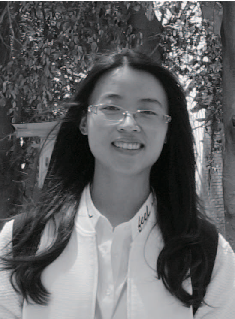
\includegraphics[width=1in,height=1.25in,clip,keepaspectratio]{bio/minlu}}]{Min lu} is an associate researcher at ShenZhen University. Her major research interest is data visualization and visual analytics, especially focusing on the urban data. She received Ph.D degree in Computer Science from Peking University in 2017 and BS degree in Computer Science from Beijing Normal University in 2011.
\end{IEEEbiography}

\begin{IEEEbiography}[{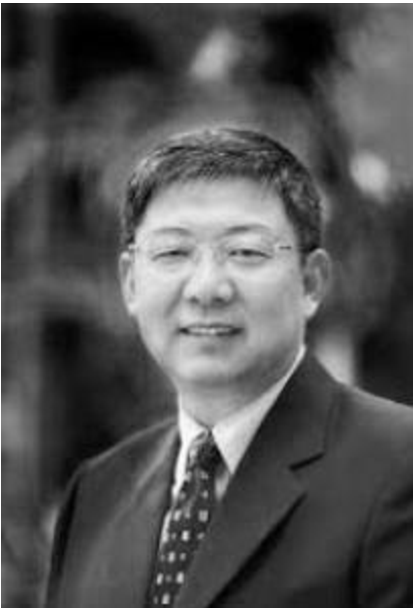
\includegraphics[width=1in,height=1.25in,clip,keepaspectratio]{bio/lqq}}]{Qingquan Li} received the Ph.D. degree in geographic information system (GIS) and photogrammetry from Wuhan Technical University of Surveying and Mapping, Wuhan, China, in 1998. He is currently a Professor with Shenzhen University, Guangdong, China, and Wuhan University, Wuhan, China. His research areas include 3-D and dynamic data modeling in GIS, location-based service, surveying engineering, integration of GIS, Global Positioning System and remote sensing, intelligent transportation system, and urban informatics.
\end{IEEEbiography}

\EOD

\end{document} 